\chapter{Project Loom}
\label{cha:ProjectLoom}

\section{Überblick}                                         % 1-2 Seiten
\label{sec:Überblick}

    Projekt Loom wurde 2017 von Ron Pressler ins Leben gerufen und ist ein Open-Source-Projekt, 
    das sich auf die Verbesserung der \gls{jvm} konzentriert. Das Ziel von Project Loom ist es, 
    die \gls{jvm} so zu erweitern, dass der Aufwand für das Schreiben, Warten und Überwachen von hochdurchsatzfähigen nebenläufigen Anwendungen,
    die die verfügbare Hardware optimal nutzen, drastisch reduziert wird \cite{ProjectLoom}.

    Die wichtigste Neuerung sind \emph{\Glspl{vt}}.
    Diese virtuelle Threads sind Threads, die im Gegensatz zu \Glspl{pt} von der JVM verwaltet werden und nicht direkt vom Betriebssystem. 
    Sie sind leichtgewichtiger als normale Threads, da sie weniger Speicher benötigen und schneller erstellt werden können \cite{JEP444}.
    Virtuelle Threads sind auch als "Continuations" bekannt und werden in anderen Programmiersprachen wie Python, Ruby und JavaScript verwendet.
    Project Loom soll die JVM so erweitern, dass sie virtuelle Threads unterstützt und Entwicklern eine einfachere Möglichkeit bietet,
    nebenläufige Anwendungen zu erstellen. Virtuelle Threads sollen die Leistung von Java-Anwendungen verbessern, indem sie die Anzahl der \Glspl{pt} reduzieren und 
    die Verwaltung von Threads vereinfachen. 

    Aufbauend darauf wird auch \emph{Strukturierte Nebenläufigkeit (Structured Concurrency)} vorgestellt.
    \texttt{StructuredTaskScope}s sollen eine Gruppe von Threads, die parallel ausgeführt werden, aber verwandte Aufgaben erledigen, als eine Arbeitseinheit behandeln. 
    Dabei soll keine Sicherheit oder Kontrolle über die einzelnen Aufgaben eingebüßt werden, sondern Kontrolle über das Gesamtverhalten der Gruppe gewonnen werden.
    Dies soll eine parallele Ausführung von verschiedenen Aufgaben einfacher gestalten und die Fehlersuche erleichtern.
    Im Hintergrund kommen dafür \Glspl{vt} zum Einsatz. \cite{JEP453}

    \emph{Bereichsgebundene Werte (Scoped Values)} sind Werte, deren Gültigkeitsbereich nach belieben festgelegt werden kann.
    Auch Verschachtelungen der Bereiche oder das
    Zuweisen verschiedener Werte auf verschiedenen Threads, ähnlich zu \texttt{ThreadLocal<>}, sind möglich. Ihre Effizienz wurde auf \Glspl{vt} optimiert.
    \cite{JEP481}
    Project Loom ist ein laufendes Projekt und manche Funktionalitäten sind noch als Preview-Funktionalität eingestuft und können in späteren Versionen Änderungen 
    unterzogen werden oder sogar wieder entfernt werden.

    

\section{Virtuelle Threads}                                 % 5 Seiten ---------------------------------------------------------------------------------------------------------
\label{sec:VirtuelleThreads}



\subsection{Was sind Virtuelle Threads?}
\label{subsec:WassindVTs?}

    Im Gegensatz zu dem bisherigen Threadmodell von Java hängt die Implementierung von \Glspl{vt} nicht so stark von den \Glspl{ot} ab. Sie führen zwar noch Code 
    auf diesen aus aber binden diesen nicht mehr ihre gesamte Lebenszeit lang an sich, im Gegensatz zu den herkömmlichen \Glspl{pt}. Dies hat zur Folge, 
    dass mehrere \Glspl{vt} Aufgaben zeitversetzt auf ein und demselben \gls{ot} ausführen können und die maximale Anzahl der \Glspl{vt}
    die maximale Anzahl von \Glspl{ot} überschreiten kann.
    Virtuelle Threads werden aber nicht direkt auf OS Threads aufgesetzt, sondern auf Plattform Threads.
    Daher werden diese auch oft als "Carrier Threads" bezeichnet.
    \cite{ieee2022}

    \begin{figure}[H]
        \centering
        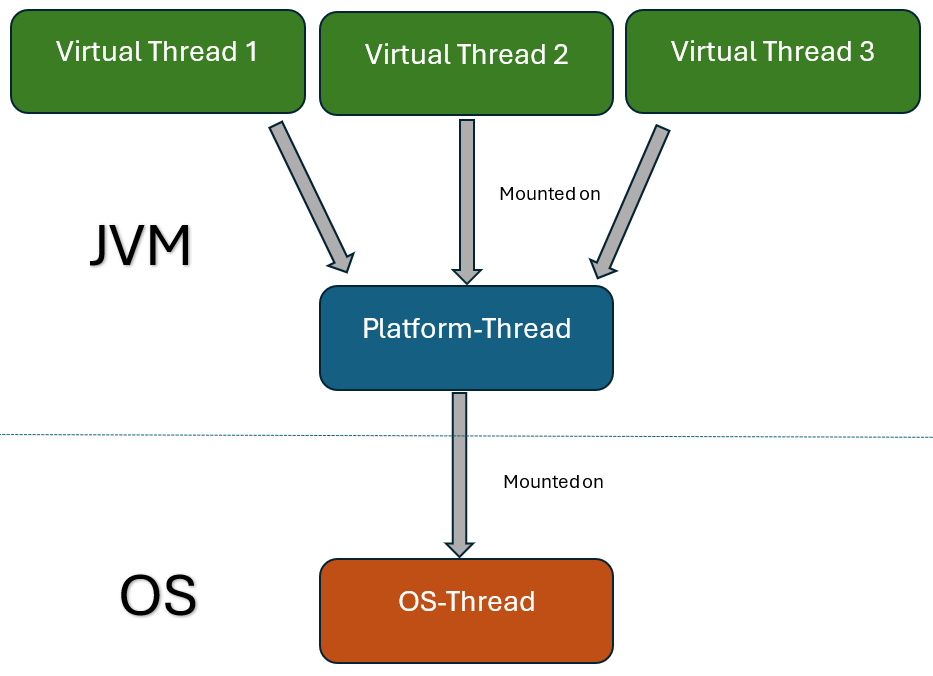
\includegraphics[width=0.6\textwidth]{VTs}
        \caption{Virtuelle Threads in der JVM}
        \label{fig:VTs}
    \end{figure}

    Da \Glspl{vt} vollkommen von der \gls{jvm} verwaltet werden und diese über die Art von Aufgabe und derzeitigen Zustand des Threads Bescheid weiß, kann die
    \gls{jvm} einen \gls{vt} von dem ihm zugeteilten \gls{pt} temporär lösen und einen anderen \gls{vt} darauf Code ausführen lassen, da das Blockieren von \Glspl{vt}
    sehr billig ist. Dies hat zur Folge, dass \Glspl{vt} nur dann Rechenzeit erhalten, wenn sie auch benötigt wird. Somit wird der Durchsatz an Recheninstruktionen
    eines \gls{pt} stark erhöht.
    Wird aber nur ein einzelner Thread benötigt, können diese Vorteile nicht genutzt werden. Der \gls{pt}, dem der \gls{vt} zugewiesen wurde, bindet den \gls{ot} auch
    an sich, selbst wenn kein \gls{vt} Code ausführt.
    \cite{JEP444}

    \begin{figure}[H]
        \centering
        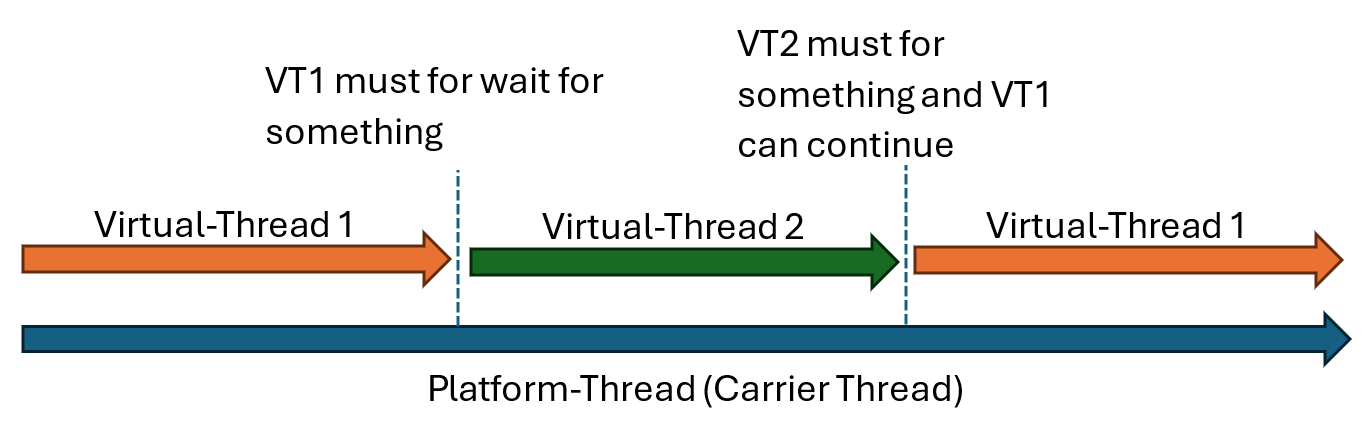
\includegraphics[width=0.67\textwidth]{VT_Coroutine}
        \caption{Coroutine von \Glspl{vt}}
        \label{fig:VT_Coroutine}
    \end{figure}

    Die \gls{jvm} kann auch die initiale Ressourcenzuweisung bei \Glspl{vt} viel präziser durchführen als das Betriebssystem bei \Glspl{ot} die mit jedem neuen \gls{pt}
    erstellt werden. Durch die enge Bindung eines \GLSpl{pt} an seinen \gls{ot} wird der Speicher für den Stack bei der Erstellung des Threads festgelegt.
    Eine dynamische Veränderung der Größe wird nicht unterstützt. Übersteigt die benötigte Größe des Stacks den Vorgaben der \gls{jvm}, wird ein \texttt{StackOverflowError}
    geworfen \cite{jvmSpecification}. Diese initiale Größe kann mit der Option \texttt{-Xss"gewünschte Größe"} für die Ausführung der \gls{jvm} verändert werden wobei 
    je nach Betriebssystem und \gls{jvm} auch hier Einschränkungen gelten oder im Konstruktor des Threads mitgegeben werden. Da das Betriebssystem nicht weiß wie spezifische Programmiersprachen ihren Stack verwalten, allokiert
    es den Speicher für den Stack eher großzügig \cite{ProjectLoom}.
    \Glspl{vt} hingegen speichern ihren Stack als \texttt{stack chunk object} im Heap ab. Diese können zur Laufzeit wegen ihrer losen Bindung zu \Glspl{ot},
    dynamisch ihre Größe ändern. 
    Im Gegensatz zu \Glspl{pt} sind \Glspl{vt} auch keine "GC-roots", also Startobjekte für den Speicherfreigabe-Prozess. Alle nicht durch GC-roots erreichbaren
    Objekte werden vom "Garbage Collector" freigegeben. Dadurch werden die in \Glspl{vt} enthaltenen
    Referenzen nicht vom Garbage Collector durchwandert. Wird beispielsweise ein \gls{vt} durch ein \texttt{BlockingQueue.take} blockiert und kein anderer Thread eine
    Referenz auf den \gls{vt} oder die \texttt{BlockingQueue} besitzt, wird der \gls{vt} freigegeben. Dies ist erwünschtes Verhalten, da dieser in diesem Fall 
    nicht wieder entblockt werden kann. Sollte der \gls{vt} aber laufen oder ein anderer Thread eine Referenz auf die \texttt{BlockingQueue} enthalten ist der 
    \gls{vt} über die GC-root des \gls{pt} erreichbar und bleibt bestehen \cite{JEP444}.
    Vor allem bei Anwendungen, die viele Threads über einen längeren Zeitraum  laufen lassen, trägt das Verhalten von \GLSpl{vt} zur Effizienz und Stabilität bei.
    Ansonsten unterscheiden sich \Glspl{vt} nicht stark von \Glspl{pt} und werden von den gleichen Problemen geplagt wie beispielsweise Deadlocks, Race Conditions\cite{JEP425}.


\subsection{Wie werden VTs benutzt?}
\label{subsec:WieWerdenVTsBenutzt?}

    Die Erstellung und Verwendung von virtuellen Threads unterscheidet sich nicht stark von den Platform-Threads. 
    \begin{program} [H]
        \caption{Erstellung eines \Glspl{vt}}
        \label{prog:ErstellungEinesVT}
        % \begin{JavaCode}
    \begin{JavaCode}[language=Java, numbers=left]
public static void main(String[] args) {
    Thread vt = Thread.ofVirtual().name("VirtualThread").unstarted(() -> {
        System.out.println("Hello from a virtual thread!");
    });
    vt.setPriority(Thread.MAX_PRIORITY);
    vt.start();
    Thread vt1 = Thread.startVirtualThread(() -> {
        System.out.println("Hello from another virtual thread!");
    });
    try {
        vt.join(); vt1.join();
    } catch (InterruptedException e) {
        e.printStackTrace();
    }
}\end{JavaCode}
    \end{program}
    Anstatt \texttt{new Thread(Runnable task).start();} wird der Ausdruck aus Zeile 2 in Programm 
    \ref{prog:ErstellungEinesVT} benutzt um einen neuen Thread zu erstellen. Dabei kann der \texttt{unstarted} Methode ein \texttt{Runnable} mitgegeben werden um den Thread später mit \texttt{start} zu starten. Alternativ kann auch ohne der 
    \texttt{unStarted} Methode \texttt{.start(Runnable r)} aufgerufen werden um den Thread sofort zu starten. Sollte ein \gls{vt} sofort gestartet werden, kann auch \texttt{startVirtualThread} wie in Zeile 9 benutzt werden. Diese Methode nimmt ebenfalls ein
    \texttt{Runnable} als Parameter. \texttt{Thread.join()} lässt genauso wie bei \Glspl{pt} den aktuellen Thread 
    auf die Beendung des Threads warten, für den \texttt{.join()} aufgerufen wurde. Die Nachteile dieser Art der Verwendung sind Codeduplizierung und erhöhter Aufwand
    beim Starten mehrerer Threads, da Eigenschaften wie der Name für jeden Thread individuell angepasst werden müssen. Typische Anwendungsfälle sind schnelle
    einmalige Aufgaben, die sofort und ohne große Konfiguration ausgeführt werden sollen \cite{oracle21Thread}.
    Weiters besteht auch die Möglichkeit einen \texttt{Thread.Builder} zu benutzen, der die Anpassung solcher Eigenschaften wie eine Zeichenkette und fortlaufende Zahl
    als Name selbständig weiterführt.
    Bei \Glspl{pt} verändert \texttt{.setPriority(int)} je nach Betriebsystem und Implementierung der \gls{jvm} die Priorität des Threads im Prozess-Scheduler. Bei \Glspl{vt} ist dieser Methodenaufruf in Java 21 zwar
    möglich, hat aber keine Auswirkungen da die Priorität auf \texttt{NORM\_PRIORITY} fixiert wurde. Dies könnte sich aber in zukünftigen Versionen ändern \cite{JEP444}.

    
    \begin{program} [H]
        \caption{Beispiel eines \texttt{Thread.Builder.OfVirtual} in Java}
        \label{prog:ErstellungEinesVTBuilders}
    \begin{JavaCode}[language=Java, numbers=left]
public static void main(String[] args) {
    try {
        Thread.Builder builder = Thread.ofVirtual().name("worker-", 0);
        Runnable task = () -> {
            // do something
        };
        // name "worker-0"
        Thread t1 = builder.unstarted(task);
        t1.setPriority(Thread.MAX_PRIORITY);    //Priority is set for each Thread 
                                                //individually   
        t1.start(); t1.join();
        System.out.println(t1.getName() + " terminated");
        // name "worker-1"
        Thread t2 = builder.start(task);   
        t2.join();  
        System.out.println(t2.getName() + " terminated");
    } catch (InterruptedException e) {
        e.printStackTrace();
    }
}\end{JavaCode}
    \end{program}

    Dabei können Regeln für verschiedene Attribute wie eine Namenskonvention
    in einem Schritt für alle späteren Threads festgelegt werden, was Codeduplizierung entgegenwirkt.
    Die Methode \texttt{name(String, long)} ermöglicht eine automatisierte fortlaufende Benennung zukünftig erstellten Threads. Wie wie in Zeile 3 in Programm \ref{prog:ErstellungEinesVTBuilders} zu sehen nimmt die Methode einen Präfix in Form einer Zeichenkette und einen Startwert vom primitiven
    Datentypen \texttt{long}. Der erste durch den Builder erstellte Thread als Namen eine Konkatinierung des Präfixes und des Startwertes. Bei jedem weiteren Thread wird der Startwert um eins inkrementiert. Lässt man den Startwert als Methodenparameter weg, heißen alle Threads gleich 
    \cite{oracle22Builder}. 

    \begin{program} [H]
        \caption{Example of a virtual threadexecutor in Java}
        \label{prog:ErstellungEinesExecutors}
    \begin{JavaCode}[language=Java, numbers=left]
public static void main(String[] args) {
    try (var executor = Executors.newVirtualThreadPerTaskExecutor()){
        IntStream.range(0, 1000).forEach(i -> {
            executor.execute(() -> {     //.submit() returns a Future<> object that can be used to retrieve the result of a computation; .execute() does not return a result.
                System.out.println("Thread " + i + " started");
            });
        });
    }       // executor.close() is called is called implicitly and the Thread waits for all tasks to finish
    System.out.println("All Tasks finished"); 
}\end{JavaCode}
    \end{program}

    Wird eine große Anzahl an \Glspl{vt} benötigt,  ist ein Executor bzw. Threadpool empfehlenswert. Dieser sollte in Kombination mit einem
    try-with-resources-Block verwendet werden, da dieser beim Verlassen des Blockes implizit geschlossen wird. Wird dies nämlich nicht gemacht kann es
    im Falle einer Ausnahme dazu kommen dass ein Thread nicht beendet wird und und weiterhin im Hintergrund Systemressourcen verschwendet.
    Dabei spricht man von einem \texttt{Thread-Leck}. Der \texttt{.newVirtualThreadPerTaskExecutor()}
    erstellt im Gegensatz zum \texttt{.newFixedThreadPool()} für jede Aufgabe einen neuen \gls{vt}.
    Sollten die Aufgaben einen Wert retournieren muss anstatt \texttt{execute} die Methode \texttt{submit} benutzt werden. Dies retourniert ein \texttt{Future<T>}Objekt 
    \cite{oracle21VritualThreads}.
    Der von der \texttt{Future} enthaltene Wert kann mit der
    \texttt{get}  Methode ausgelesen werden. Dabei handelt es sich um eine blockierende Instruktion. Daher wird die Ausführung des Eltern-Threads bis zur
    Beendung des Kind-Threads angehalten \cite{oracle21Future}.
    


\section{Structured Concurrency}                                 % 4 Seiten ---------------------------------------------------------------------------------------------------------
\label{sec:Structured Concurrency}


\subsection{Was ist Structured Concurrency?}
\label{subsec:WasistSC?}
    Der Bereich \emph{strukturierte Nebenläufigkeit (Structured Concurrency)} in Project Loom fügt \texttt{\Glspl{sts}} zur Standartbibliothek von Java hinzu
    und befindet sich derzeit noch in
    aktiver Entwicklung. Das heißt, dass sich verschiedene Funktionalitäten ändern oder wieder entfernt werden können.
    Die zu strukturierten Nebenläufigkeit gehörigen Klassen ermöglichen
    es, eine Gruppe von parallelen Teilaufgaben als eine Einheit zu koordinieren. Allgemeine Ausführungslogik und Fehlerbehandlung kann dadurch schon vorher festgelegt und 
    wiederverwendet werden.
    Wie der Name bereits verrät, wird dabei ein Block festgelegt, in dem diese Teilaufgaben erstellt und behandelt werden.
    Dadurch müssen die Teilaufgaben vor dem Hauptprozess, in dem sie gestartet wurden, beendet werden.
    \cite{oracle21SC}

    \begin{program} [H]
        \caption{Beispiel für einen einfachen \gls{sts}}
        \label{prog:BeispielFürEinenEinfachenSts}
    \begin{JavaCode}[language=Java, numbers=left]
public static void main(String[] args) {
    try (var scope = new StructuredTaskScope<>()) {
        StructuredTaskScope.Subtask<String> result1 = scope.fork(() -> {
            Thread.sleep(1000);
            return "Result from task 1";
        });
        var result2 = scope.fork(() -> {
            Thread.sleep(2000);
            throw new RuntimeException("Task 2 failed");
        });
        StructuredTaskScope.Subtask<Integer> result3 = scope.fork(() -> {
            Thread.sleep(3000);
            return 3;
        });
        scope.join();                        // Waits for all subtasks to complete
        if (result1.state() == StructuredTaskScope.Subtask.State.SUCCESS){
            System.out.println(result1.get());  
        } 
        System.out.println(result2.get());   // Throws an IllegalStateException
        System.out.println(result3.get());
    } catch (Exception e) {                 // calls .close() implizit.
        e.printStackTrace();
    }
}\end{JavaCode}
    \end{program}
    Wird der \gls{sts} ohne Typ erstellt können die einzelnen Teilprozesse Objekte verschiedener Typen returnieren. \texttt{new StructuredTaskScope<Integer>()}
    hätte beispielsweise eine einschränkende Wirkung.
    Es wird stark empfohlen, einen \gls{sts} in Form eines try-with-resources-Blocks zu realisieren, da dieser den Gültigkeitsbereich wieder schließt. In diesem Block
    werden Teilaufgaben mit der Methode \texttt{.fork(Runnable r)} erschaffen. Diese haben den Rückgabewert \texttt{StructuredTaskScope.Subtask<T>}, wobei sie keine
    primitiven Datentypen aufnehmen können. Mit \texttt{.state()} kann überprüft werden, ob die einzelnen Ausführungen erfolgreich waren.
    Wichtig dabei ist der Aufruf von \texttt{.join()}. Dadurch wartet der \gls{sts}, darauf dass entweder alle Teilprozesse beendet werden oder fehlschlagen, oder
    eine andere vordefinierte Abbruchbedingung erreicht wird.
    \cite{oracle21STS}

    \begin{program} [H]
        \caption{Beispiel für ShutdownOnFailure}
        \label{prog:BeispielFürShutdownOnFailure}
    \begin{JavaCode}[language=Java, numbers=left]
public static void main(String[] args) {
    StructuredTaskScope.Subtask<String> result1 = null;
    StructuredTaskScope.Subtask<String> result2 = null;
    StructuredTaskScope.Subtask<String> result3 = null;
    try (var scope = new StructuredTaskScope.ShutdownOnFailure()) {            // shuts down the scope if a subtask fails
        result1 = scope.fork(() -> {
            Thread.sleep(1000);
            return "Result from task 1";
        });
        result2 = scope.fork(() -> {         // used to return a Future<> object
            Thread.sleep(2000);
            throw new RuntimeException("Task 2 failed");
        });
        result3 = scope.fork(() -> {
            Thread.sleep(5000);
            return "Result from task 3";
        });
        scope.join().throwIfFailed();
    } catch (Exception e) {
        System.out.println("Scope failed");
    }
    System.out.println(result1.get());                                          
    System.out.println(result2.get());         //Throws an IllegalStateException
    System.out.println(result3.get());        // Throws an IllegalStateException due to the exception in the second task
}\end{JavaCode}
    \end{program}
    Eine der zwei abgeleiteten verschachtelten Unterklassen ist \texttt{ShutdownOnFailure}. Sie ist mit \texttt{final} markiert und steht damit nicht für weitere
    Vererbung zur Verfügung. Der Hauptunterschied zur Basisklasse besteht darin, dass die Ausführung aller Teilprozesse beendet wird, sobald nur einer davon fehlschlägt.
    Dies hat zur Folge, dass alle noch nicht beendeten Aufgaben ebenfalls fehlschlagen und deren Ergebnisse nicht abgefragt werden dürfen. Dieses Verhalten ist besonders dann
    erwünscht wenn alle Teilergebnisse essentiell sind und das Fehlschlagen eines einzelnen Teilprozesses somit das Gesamtergebnis unbrauchbar macht. 

    \begin{program} [H]
        \caption{Beispiel für ShutdownOnSuccess}
        \label{prog:BeispielFürShutdownSuccess}
    \begin{JavaCode}[language=Java, numbers=left]
public static void main(String[] args) {
    StructuredTaskScope.Subtask<String> result1 = null;
    StructuredTaskScope.Subtask<String> result2 = null;
    String result = null;
    try (var scope = new StructuredTaskScope.ShutdownOnSuccess<String>()) {                 // shuts down the scope if a subtask succeeds
        result1 = scope.fork(() -> {
            Thread.sleep(2000);
            return "Result from task 1";
        });
        result2 = scope.fork(() -> {
            return "Result from task 2";
        });
        result = scope.join().result();      // .result() returns the result of the scope
    } catch (Exception e) {
        System.out.println("Scope failed");
        e.printStackTrace();
    }
    System.out.println(result1.get());            // Throws an IllegalStateException because the scope is shut down due to the success of the second task
    System.out.println(result2.get());
    System.out.println(result);
}\end{JavaCode}
    \end{program}
    Die zweite abgeleitete verschachtelte Unterklasse ist \texttt{ShutdownOnSuccess} und ist ebenfalls \texttt{final}. Hierbei werden die Ausführungen gestoppt, falls
    einen Teilaufgabe erfolgreich beendet wird. Eine Abfrage der Ergebnisse der Teilaufgaben ist möglich, wird aber nicht empfohlen, da es nur ein gültiges
    Ergebnis geben kann
    und dieses mit \texttt{.result()} direkt abgefragt werden kann. Dabei wird das Ergebnis direkt zurückgegeben und nicht als \texttt{StructuredTaskScope.Subtask<>}.
    Schlagen alle Teilaufgaben fehl, wird null retourniert.


    % Zitate!!!!!!!!!!!!!!!!!!!!!!!!!

\subsection{Erstellung eines eigenen \texttt{StructuredTaskScopes}}
\label{subsec:ErstellungEinesEigenenSts?}

    Nicht immer erfüllen die zwei Subklassen \texttt{ShutdownOnFailure} und \texttt{ShutdownOnSuccess} den individuellen Anforderungen des Anwenders.
    Es könnte zum Beispiel nur das Kleinste Ergebnis aller erfolgreich abgeschlossenen Aufgaben gewünscht werden oder man möchte alle Ergebnisse mit
    einem Methodenaufruf erhalten ohne sich die \texttt{Subtask<>}s abspeichern zu müssen.
    Die Klasse \texttt{StructuredTaskScopes<T>} wurde nicht mit final markiert und lässt somit Ableitungen zu. Die für die Erstellung individueller Implementierungen wichtigen
    Methoden wurden mit der Sichtbarkeit \texttt{protected} versehen und lassen sich daher nach belieben überschreiben.


    \begin{program} [H]
        \caption{Beispiel für den Aufbau von \texttt{SmallestScope<T>}}
        \label{prog:BeispielFürSmallestScope}
    \begin{JavaCode}[language=Java, numbers=left]
public class SmallestScope<T> extends StructuredTaskScope<T> {
    private final Collection<T> results = new ConcurrentLinkedDeque<>();
    private final Collection<Throwable> exceptions = new ConcurrentLinkedDeque<>();
    private final Comparator<T> comparator;

    public SmallestScope(Comparator<T> comparator) {
        this.comparator = Objects.requireNonNull(comparator);
    }

    @Override
    protected void handleComplete(Subtask<? extends T> subtask) {...}

    public Exception exceptions() {...}

    public T smallest() throws Exception {...}

    @Override
    public SmallestScope<T> join() throws InterruptedException {
        super.join();
        return this;
    }

    @Override
    public SmallestScope<T> joinUntil(Instant deadline)
        throws InterruptedException, TimeoutException{
            super.joinUntil(deadline);
            return this;
    } 
}\end{JavaCode}
    \end{program}
    
    Ein Beispiel für einen individualisierten \gls{sts} ist \texttt{SmallestScope<T>}. Dieser soll nach Beendung oder Fehlschlag aller Teilprozesse das Kleinste 
    aller Ergebnisse liefern.
    Dafür muss zunächst von von \texttt{StructuredTaskScope<T>} abgeleitet werden. Außerdem werden noch zusätzliche Datenkomponenten benötigt wie in den Zeilen 2 bis 4 in
    \ref{prog:BeispielFürSmallestScope} zu sehen ist. 
    Um die einzelnen Teilergebnisse für die weitere Verarbeitung zu speichern wird ein Behälter benötigt.
    Dieser sollte theadsicher sein da mehrere Prozesse darauf zugreifen müssen.
    Da der Benutzer an den Fehlermeldungen der Subprozesse interessiert sein könnte sollten diese ebenfalls in einem threadsicheren Behälter aufbewahrt werden. 
    Um das kleinste Ergebnis ermitteln zu können wird zunächst eine Vergleichsmöglichkeit in Form eines \texttt{Comperator<T>}-Objekts benötigt. Dieses wird über den
    Konstruktor injiziert.
    Das Überschreiben der Methoden \texttt{join()} und \texttt{joinUntil(Instant deadline)} ist nicht essentiell um die Klasse benutzen zu können sondern ermöglicht
    lediglich Methodenverkettung zu ermöglichen. Dies ist zwar nicht dringend nötig wird aber stellt für viele ein erwartetes verhalten dar.

    \begin{program} [H]
        \caption{Überschreiben von \texttt{handleComplete}}
        \label{prog:ÜberschreibenVonHandleComplete}
    \begin{JavaCode}[language=Java, numbers=left]
@Override
protected void handleComplete(Subtask<? extends T> subtask) {
    switch (subtask.state()) {
        case SUCCESS -> results.add(subtask.get());
        case FAILED, UNAVAILABLE -> {
            exceptions.add(subtask.exception());
        }
    }
}\end{JavaCode}
    \end{program}
    Die Methode \texttt{handleComplete()} wird von jedem Thread bei Beendung seiner Aufgabe aufgerufen, vorausgesetzt der \gls{sts} wurde durch z.B. der Methode 
    \texttt{shutdown()} noch nicht beendet.
    Um den gewünschten Effect zu erzielen muss zunächst der Zustand des \texttt{Subtask}s abzufragen. Beim Zustand \texttt{SUCCESS} kann das Ergebnis in den Behälter für Ergebnisse
    gespeichert werden. Ist der Zustand \texttt{FAILED} oder \texttt{UNAVAILABLE} wird die Fehlermeldung abgefragt und in dem dafür vorgesehenen Behälter platziert.

    \begin{program} [H]
        \caption{Returnieren des kleinsten Ergebnisses}
        \label{prog:ReturnierenDesKleinstenErgebnisses}
    \begin{JavaCode}[language=Java, numbers=left]
public T smallest() throws Exception {
return results.stream()
        .filter(Objects::nonNull)
        .min(comparator)
        .orElseThrow(this::exceptions);
}\end{JavaCode}
    \end{program}
    Um das kleinste Ergebnis später ermitteln und abfragen zu können wird einen neue Methode \texttt{smallest()} benötigt die nach \texttt{join()} oder
    \texttt{joinUntil(instant)} aufgerufen werden kann und das Ergebnis returniert. Dazu wird in dem Behälter mithilfe des Comperators das kleinste Element gesucht
    und zurückgegeben. Dazu wird Javas Stream-API benutzt wobei Objekte deren Wert \texttt{null} beträgt herausgefiltert werden. Sollte dies aus verschiedenen Gründen nicht möglich sein werden alle gesammelten Fehlermeldungen geworfen. 
    \begin{program} [H]
        \caption{Returnieren der Fehlermeldungen}
        \label{prog:ReturnierenDerFehlermeldungen}
    \begin{JavaCode}[language=Java, numbers=left]
public Exception exceptions() {
    Exception exception = new Exception();
    this.exceptions.forEach(exception::addSuppressed);
    return exception;
}\end{JavaCode}
    \end{program}
    Um den Nutzenden zu ermöglichen, die Fehlermeldungen der fehlgeschlagenen Teilprozesse zu erhalten wird \gls{sts} um die Methode \texttt{exceptions()} erweitert.
    Diese returniert eine neue Fehlermeldung der alle Fehlermeldungen aus dem Behälter aus \ref{prog:BeispielFürSmallestScope} in Zeile 3 angehängt werden.

    \begin{program} [H]
        \caption{Beispiel für die Verwendung von \texttt{SmallestScope<T>}}
        \label{prog:VerwendungVonSmallestScope}
    \begin{JavaCode}[language=Java, numbers=left]
public static void scopesSmallest() {
    StructuredTaskScope.Subtask<Integer> result1 = null;
    Integer result = null;

    try (var scope = new SmallestScope<Integer>(Integer::compareTo)) {                                         
        result1 = scope.fork(() -> { Thread.sleep(1000); return 4; });
        scope.fork(() -> { throw new RuntimeException("Task 2 failed"); });
        scope.fork(() -> { Thread.sleep(2000); return 3; });

        result = scope.join().smallest();
        if (result1.state() == StructuredTaskScope.Subtask.State.SUCCESS) {
            System.out.println(STR."result from the 1st Thread: \{result1.get()}");
        }
        scope.exceptions().printStackTrace();
    } catch (Exception e) {
        e.printStackTrace();
    }
    System.out.println(STR."smallest result: \{result}");
}\end{JavaCode}
    \end{program}
    Wie in \ref{prog:BeispielFürSmallestScope} ersichtlich ist kann \texttt{SmallestScope} nun ähnlich wie die anderen \Glspl{sts} benutzt werden. Der Konstruktor benötigt
    aber einen Komparator, hier \texttt{Integer::compareTo} in Zeile 5, als Parameter. Teilergebnisse der einzelnen Prozesse können ebenfalls wieder abgefragt werden. Diese Abfragen
    bringen dieselben bereits besprochenen Probleme mit sich. Die einzelnen Teilprozesse müssen 
    aber auch wie bei \texttt{ShutdownOnSuccess} den gleichen Typen returnieren wie im Generika festgelegt. Da die Methode \texttt{join()} dementsprechend überschrieben
    wurde, kann die Ergebnisabfrage \texttt{smallest()} an diese gekettet werden. Für Debugging-Zwecke können alle Fehlermeldungen wie in Zeile 14 mit \texttt{exceptions()}
    erhalten werden. Sollten alle Teilprozesse fehlschlagen werden diese aber ebenfalls geworfen. 






